\documentclass[tikz,border=2pt]{standalone}
\usepackage{amsmath}
\usetikzlibrary{arrows.meta}
\begin{document}
% Babylonian method for sqrt(2) as a while loop: g_new = (g + 2/g)/2 from g = 1;
% the condition diff > tol (tol = 1e-7) is checked before each pass; after pass 5 it is FALSE.
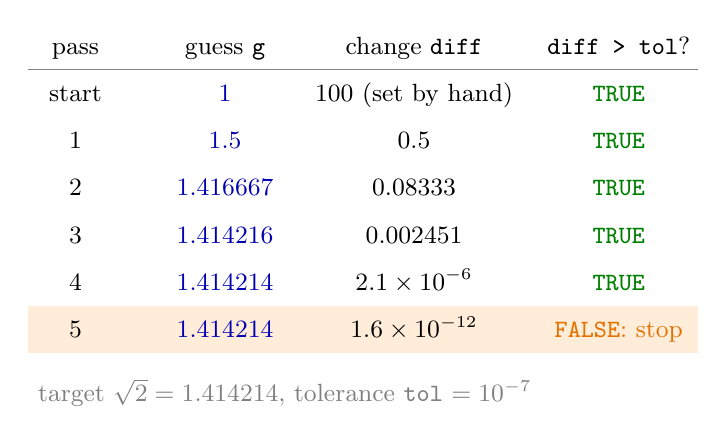
\begin{tikzpicture}[font=\small, >={Latex[length=2mm]}]
  % header
  \node[anchor=base] at (0,0)   {pass};
  \node[anchor=base] at (1.9,0) {guess \texttt{g}};
  \node[anchor=base] at (4.3,0) {change \texttt{diff}};
  \node[anchor=base] at (6.9,0) {\texttt{diff > tol}?};
  \draw[gray] (-0.6,-0.2) -- (7.9,-0.2);
  % rows
  \foreach \k/\g/\d/\c [count=\r] in {
      start/1/100 (set by hand)/TRUE,
      1/1.5/0.5/TRUE,
      2/1.416667/0.08333/TRUE,
      3/1.414216/0.002451/TRUE,
      4/1.414214/$2.1\times10^{-6}$/TRUE} {
    \node[anchor=base] at (0,-0.6*\r) {\k};
    \node[anchor=base, blue!70!black] at (1.9,-0.6*\r) {\g};
    \node[anchor=base] at (4.3,-0.6*\r) {\d};
    \node[anchor=base, green!50!black] at (6.9,-0.6*\r) {\texttt{\c}};
  }
  \fill[orange!15] (-0.6,-3.8) rectangle (7.9,-3.2);
  \node[anchor=base] at (0,-3.6) {5};
  \node[anchor=base, blue!70!black] at (1.9,-3.6) {1.414214};
  \node[anchor=base] at (4.3,-3.6) {$1.6\times10^{-12}$};
  \node[anchor=base, orange!90!black] at (6.9,-3.6) {\texttt{FALSE}: stop};
  \node[anchor=west, gray] at (-0.6,-4.3) {target $\sqrt{2}=1.414214$, tolerance \texttt{tol} $=10^{-7}$};
\end{tikzpicture}
\end{document}
